\documentclass{article}
\usepackage[utf8]{inputenc}
\usepackage{geometry}
\geometry{
	paperwidth=35cm,
	paperheight=33cm,
	top=2cm,
	bottom=2cm,
	left=2cm,
	right=2cm,
}
\usepackage{graphicx}
\graphicspath{{../plots/}}
\usepackage[font=Large,labelfont=bf]{caption}
\captionsetup{width=\linewidth}
\usepackage{subcaption}

\begin{document}

	\begin{figure}
		\centering
		\begin{subfigure} {\columnwidth}
				\centering 
				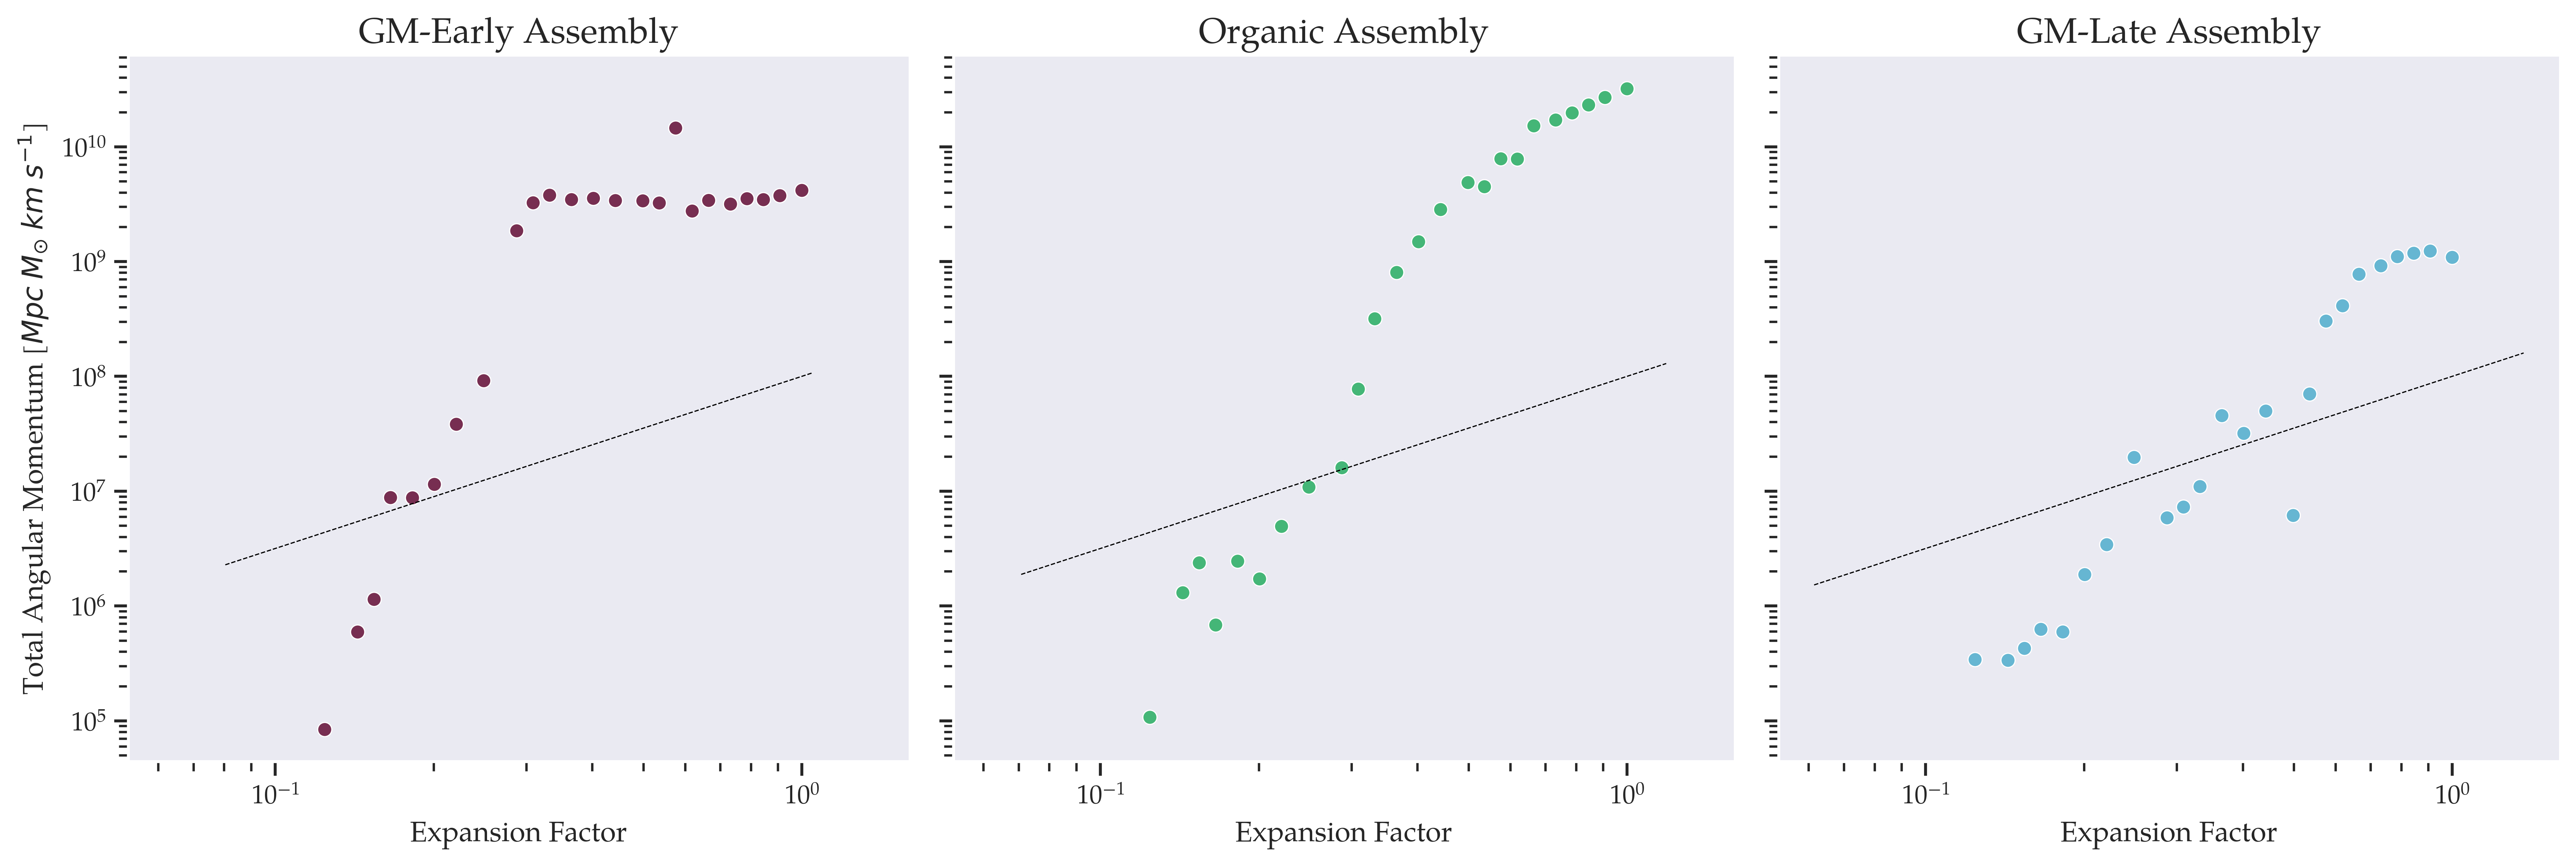
\includegraphics[width=\columnwidth]{../../plots/angular_momentum/expansion_factor-net_angular_momentum.png}
				\caption{Angular momentum vs expansion factor plot for three assembly modes.}
		\end{subfigure} \\
			% \hfill
			\vspace{1cm}
		\begin{subfigure} {\columnwidth}
				\centering 
				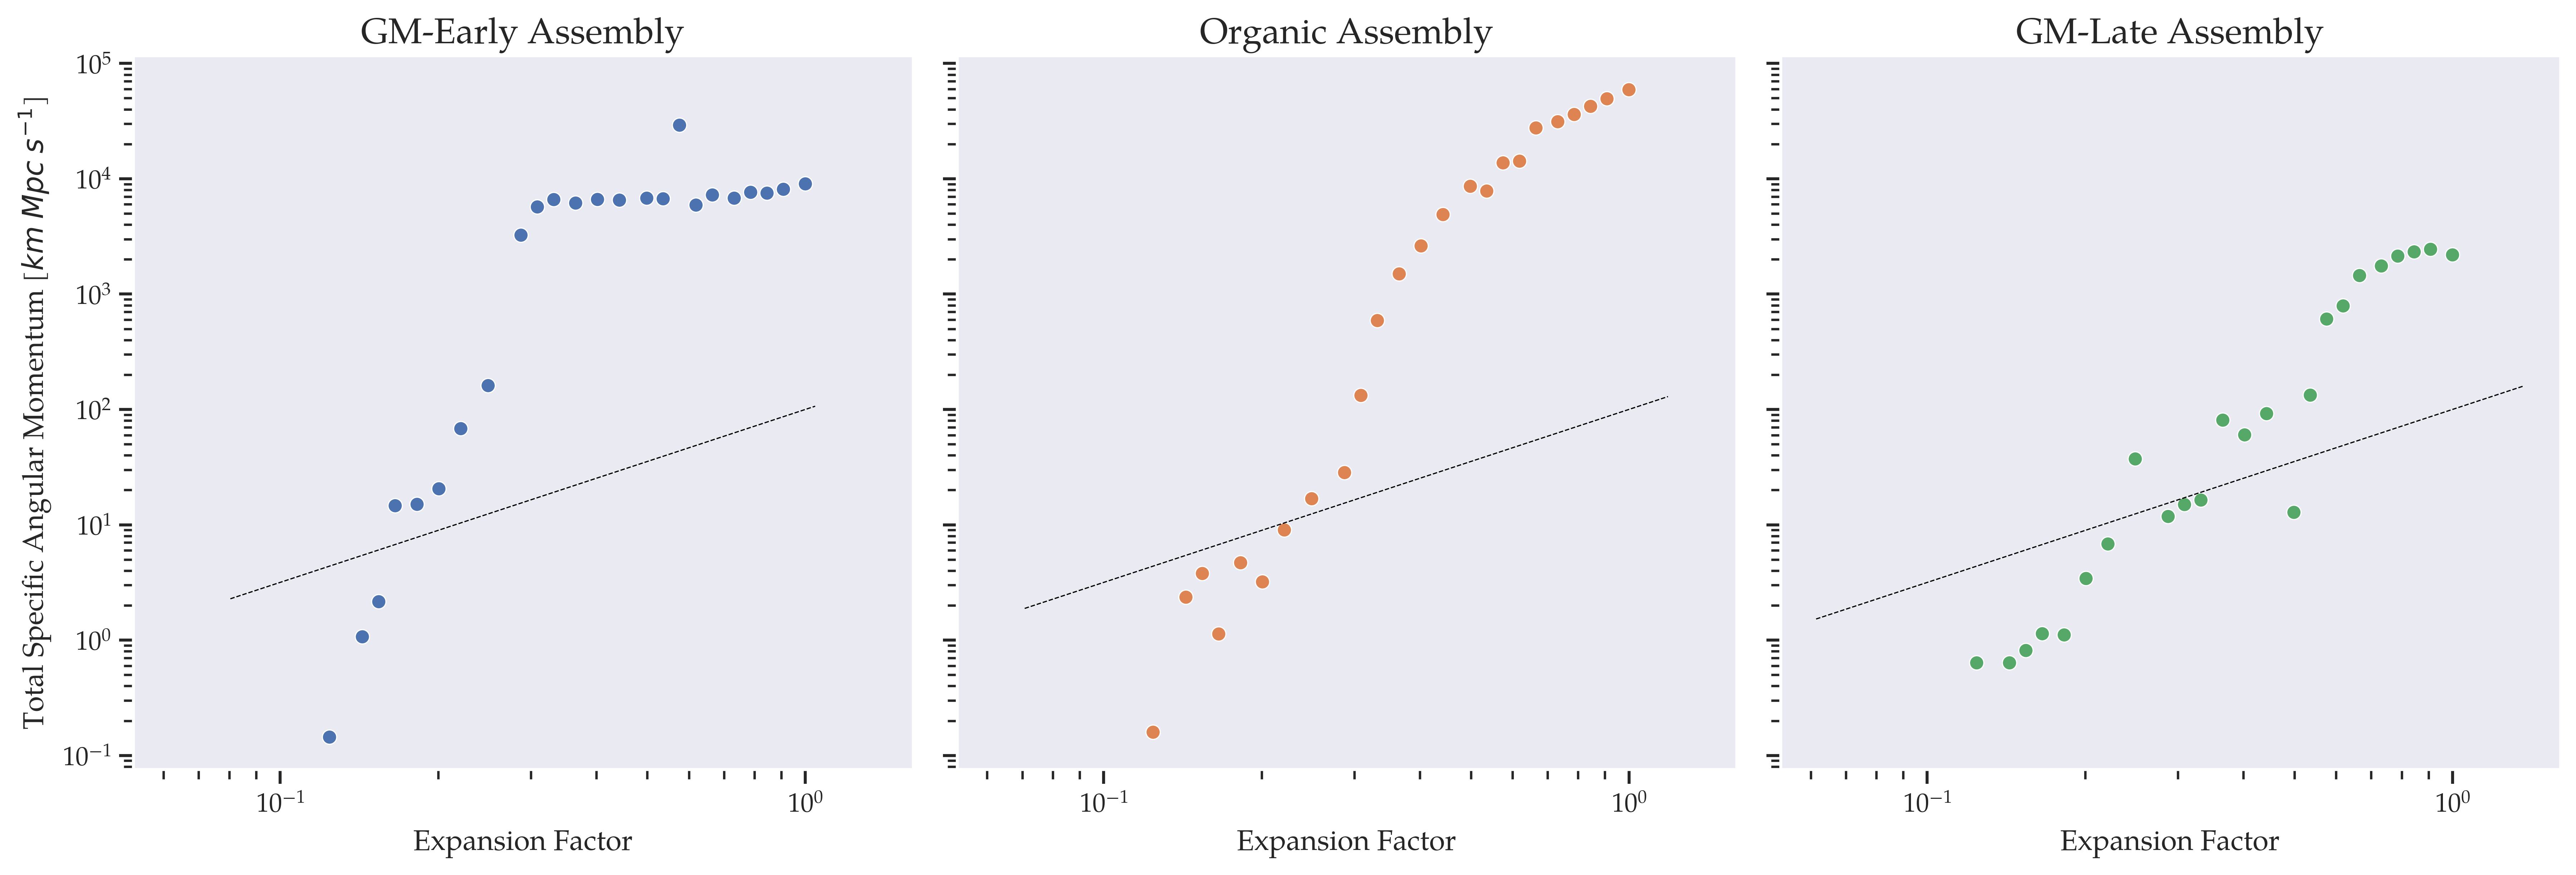
\includegraphics[width=\columnwidth]{../../plots/angular_momentum/expansion_factor-net_specific_angular_momentum.png}
				\caption{Specific angular momentum vs expansion factor plot for three assembly modes.}
		\end{subfigure}
		
		\caption{Angular momentum and specific angular momentum vs expansion factor (a) plots, overlaid by \(a^{3/2}\) dashed black line with different offsets.}
	\end{figure}

	\clearpage

	\begin{figure}
		\centering
		\begin{subfigure} {\columnwidth}
				\centering 
				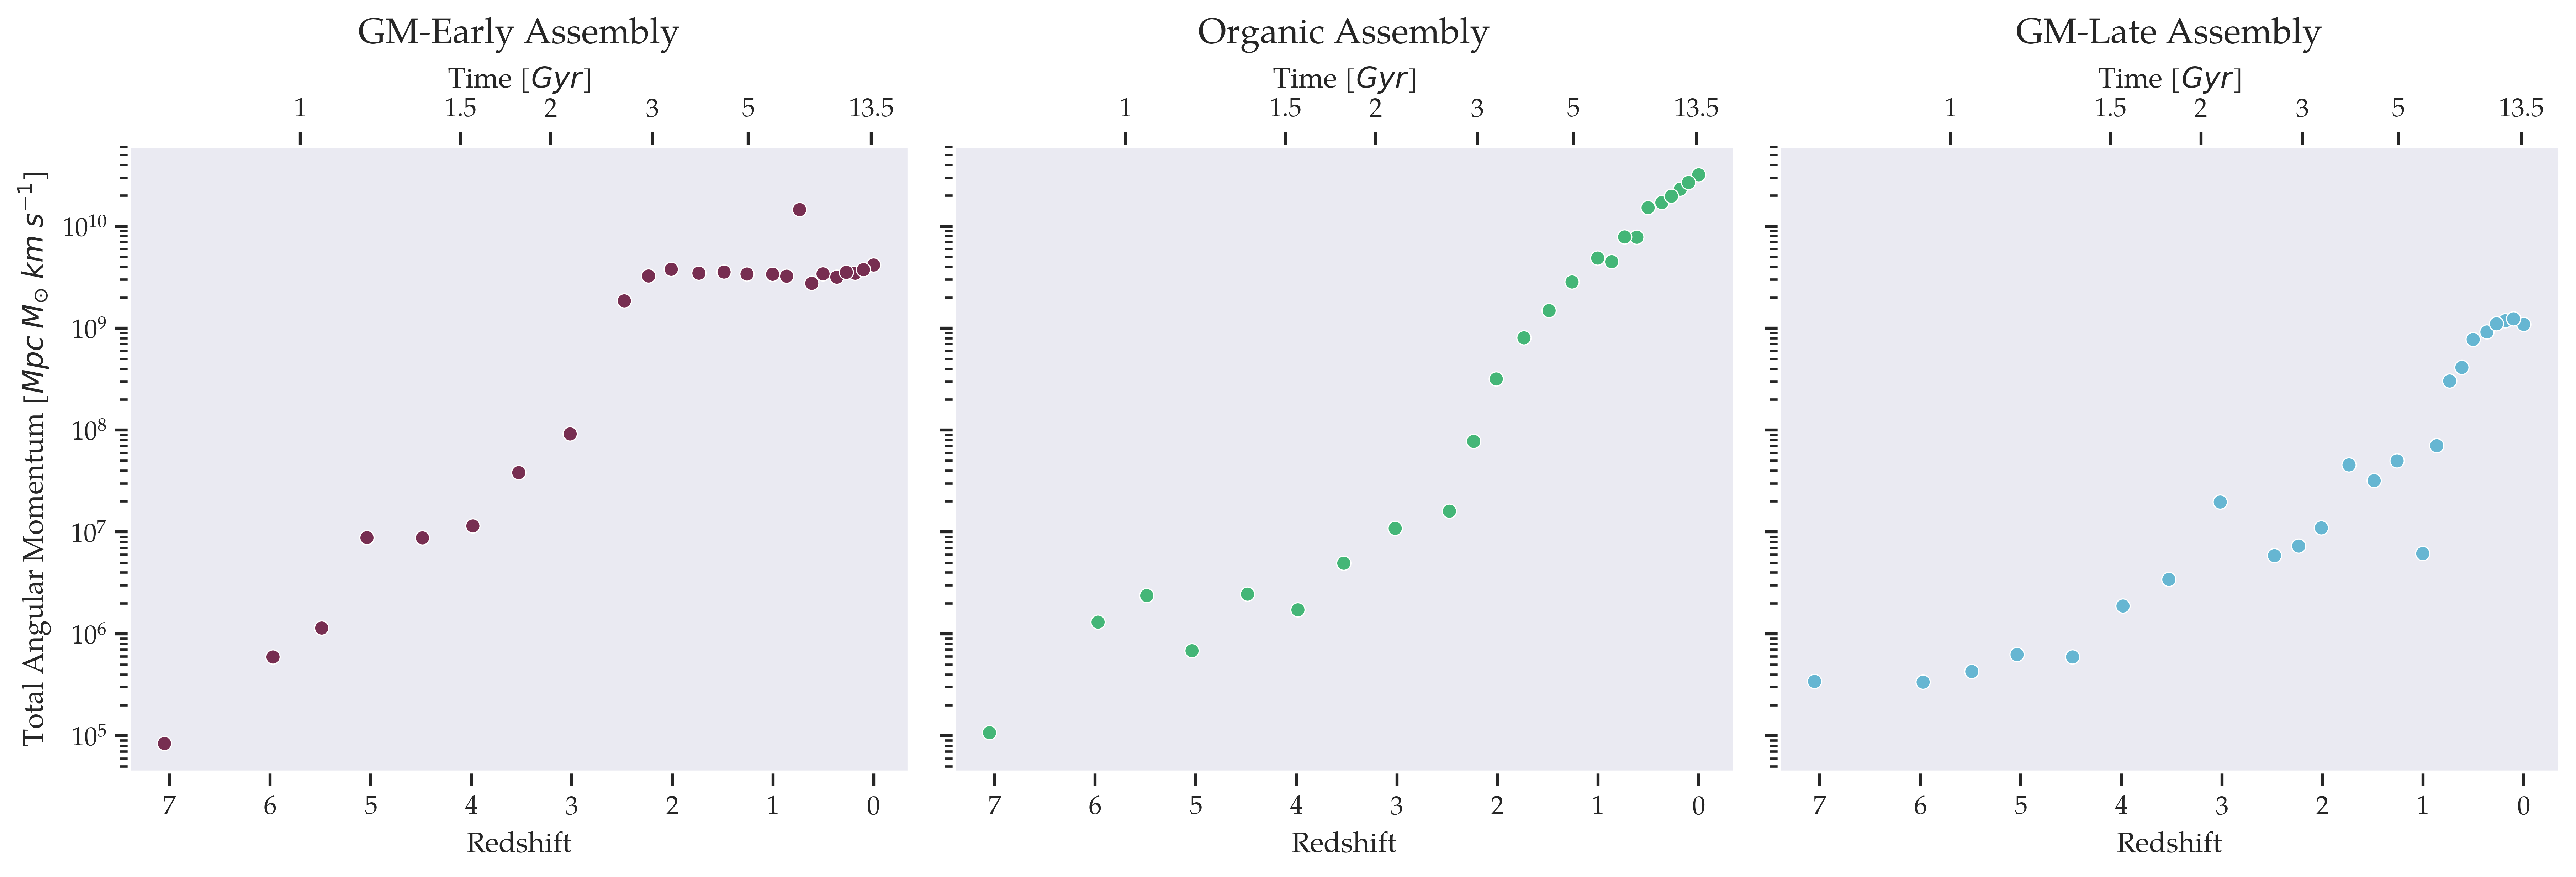
\includegraphics[width=\columnwidth]{../../plots/angular_momentum/redshift-net_angular_momentum.png}
				\caption{Angular momentum vs redshift plot for three assembly modes.}
		\end{subfigure} \\
			% \hfill
			\vspace{1cm}
		\begin{subfigure} {\columnwidth}
				\centering 
				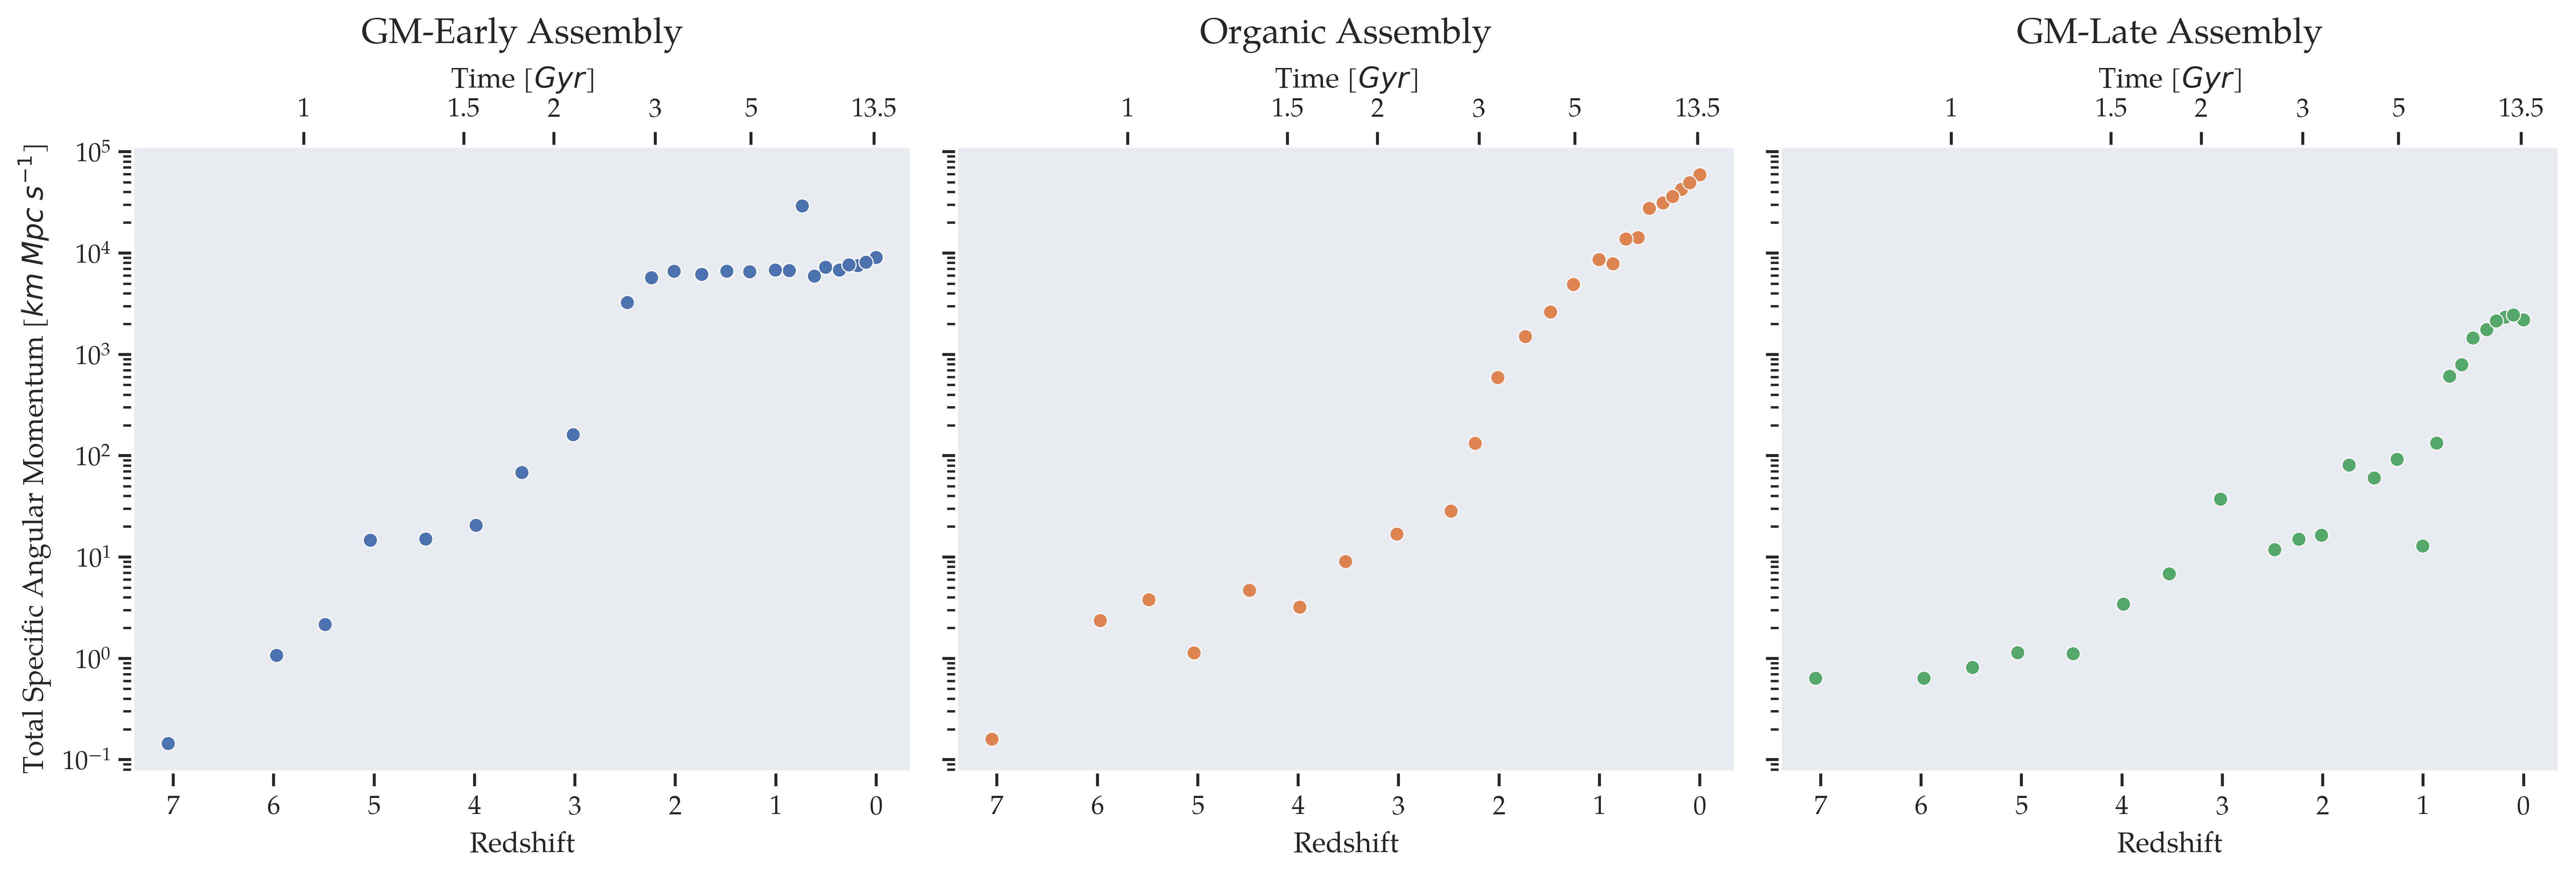
\includegraphics[width=\columnwidth]{../../plots/angular_momentum/redshift-net_specific_angular_momentum.png}
				\caption{Specific angular momentum vs redshift plot for three assembly modes.}
		\end{subfigure}
		% 	\hfill
		% \begin{subfigure} {.325\columnwidth}
		% 		\centering 
		% 		
\includegraphics[width=\columnwidth]{../../plots/angular_momentum/Organic_z-x_coordinates_evolution.png}
		% \end{subfigure}
		
		\caption{Angular momentum and specific angular momentum vs redshift plots. Time is used as a secondary x-axis.}
	\end{figure}

	\clearpage

	\begin{figure}
		\centering
		\begin{subfigure} {\columnwidth}
				\centering 
				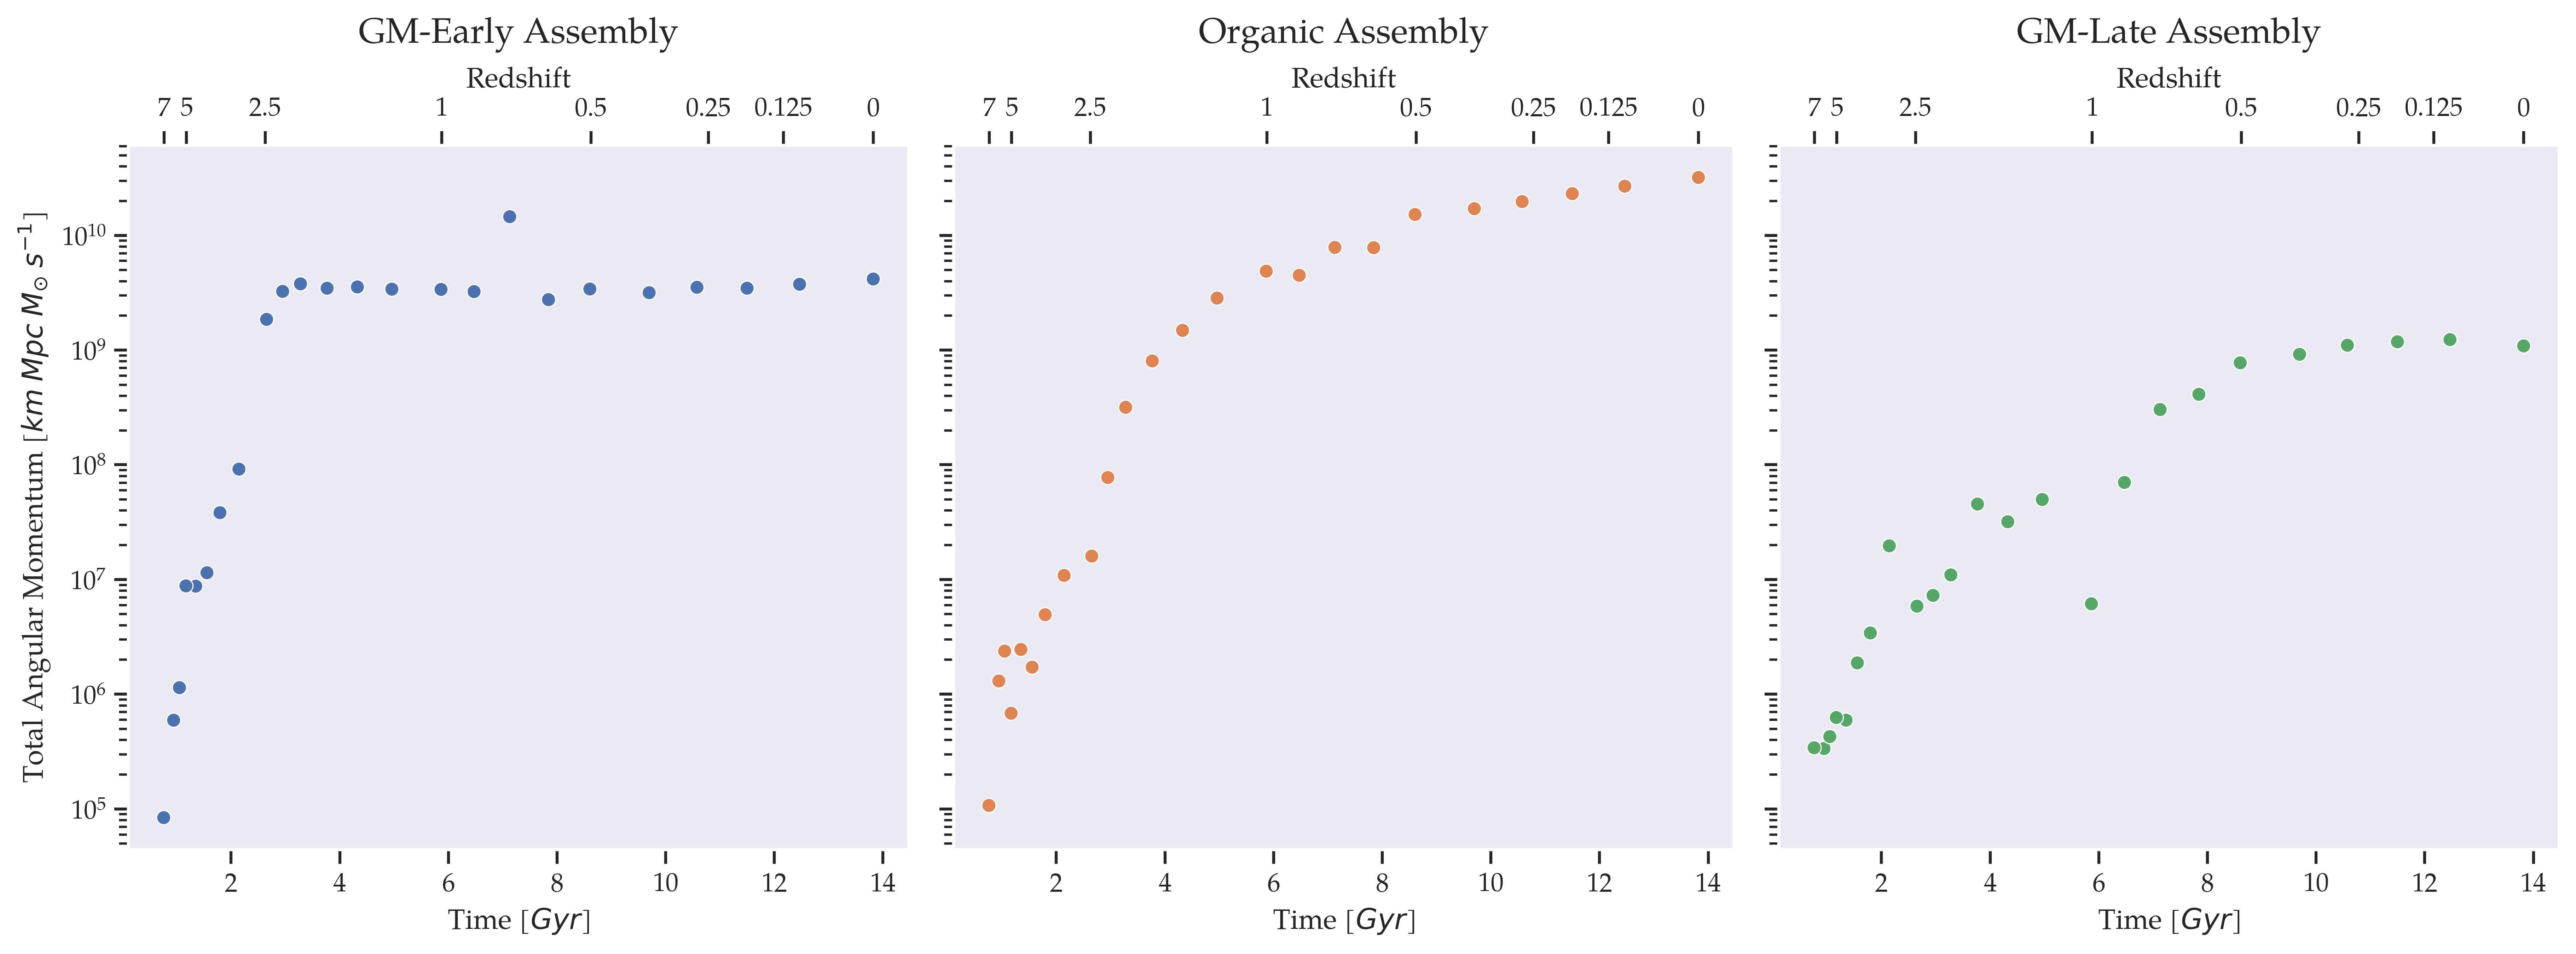
\includegraphics[width=\columnwidth]{../../plots/angular_momentum/time-net_angular_momentum.png}
				\caption{Angular momentum vs time plot for three assembly modes.}
		\end{subfigure} \\
			% \hfill 
			\vspace{1cm}
		\begin{subfigure} {\columnwidth}
				\centering 
				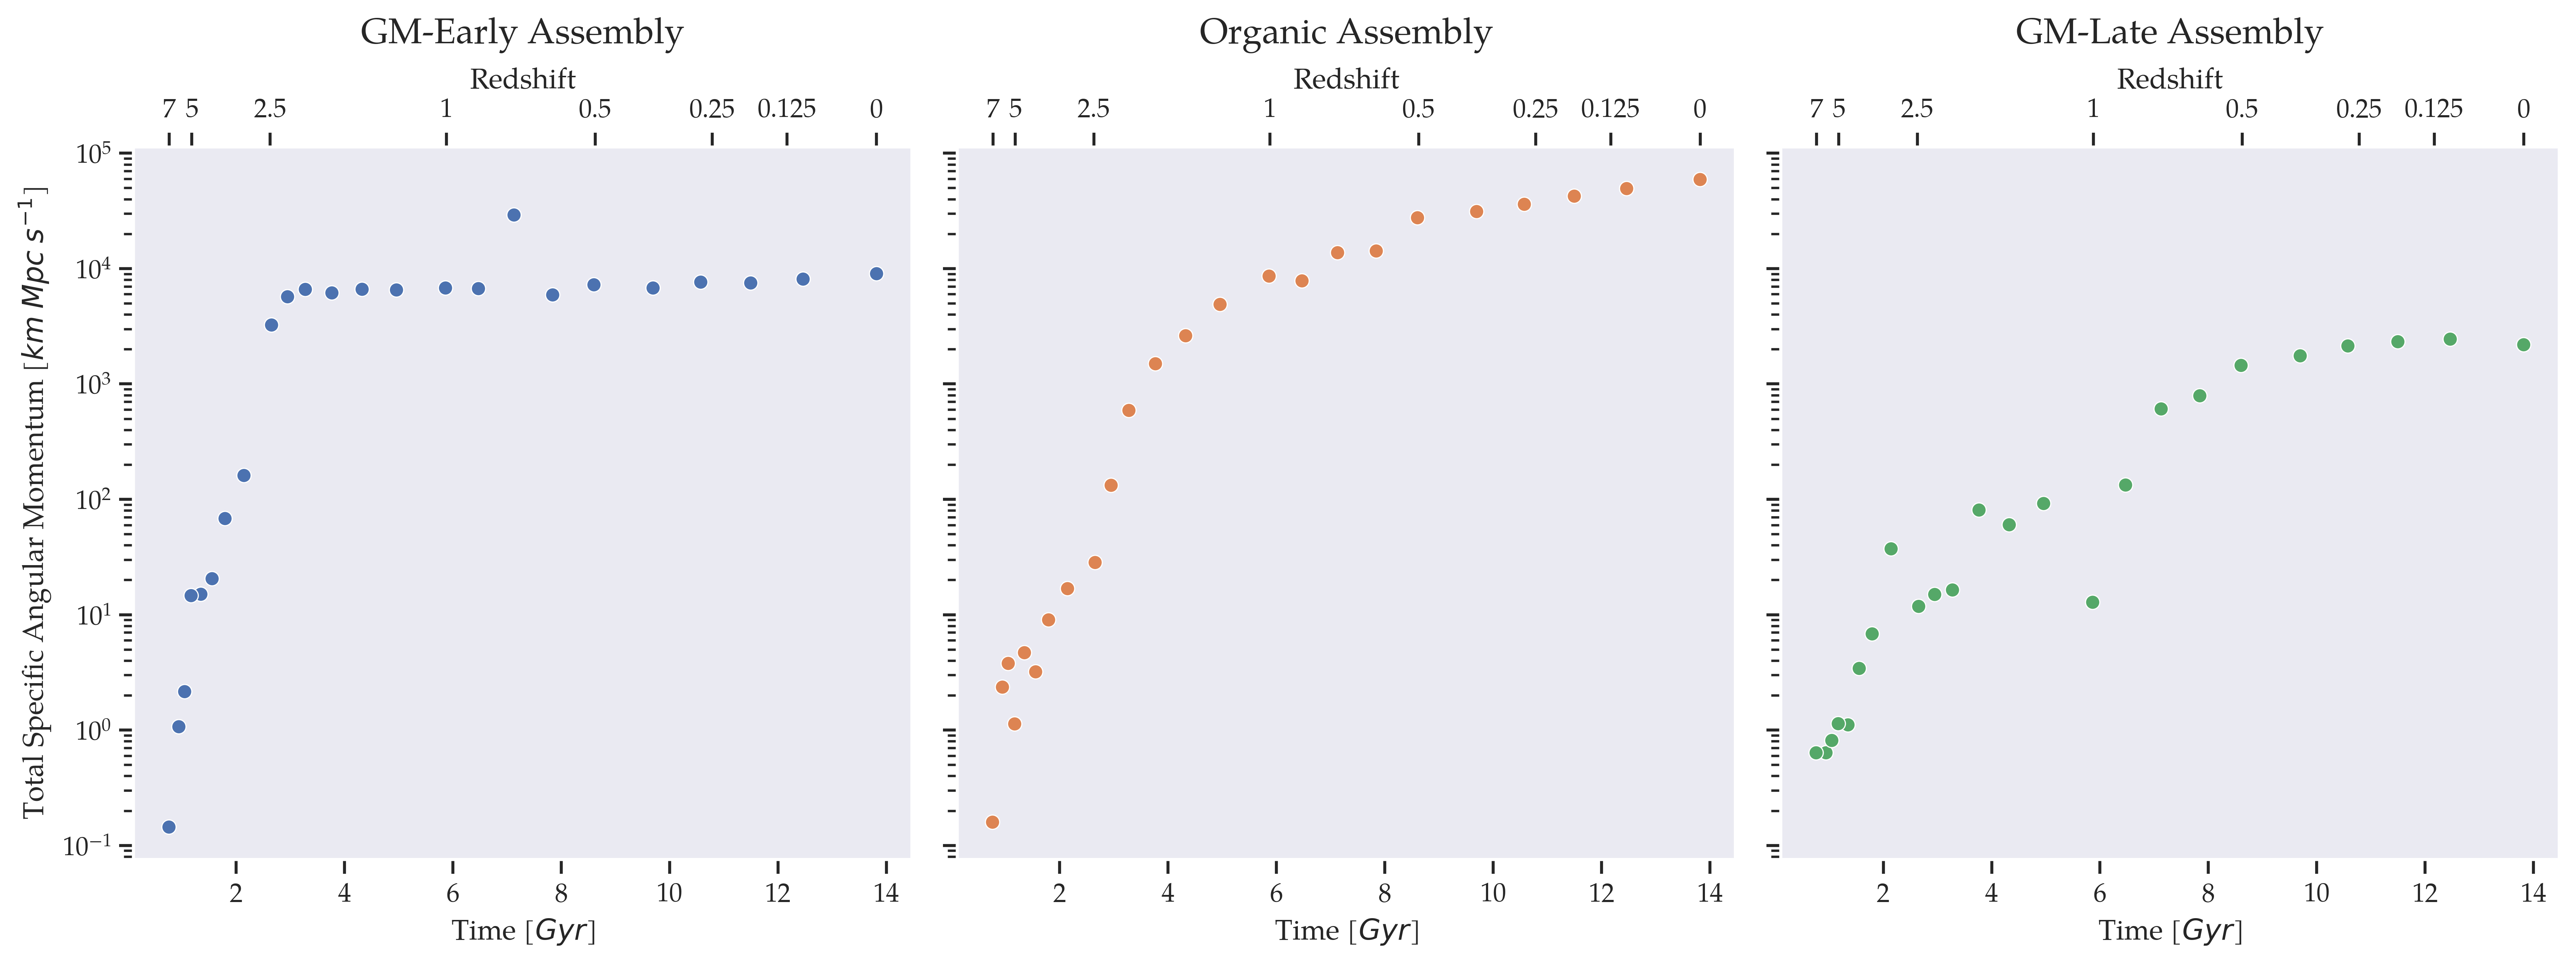
\includegraphics[width=\columnwidth]{../../plots/angular_momentum/time-net_specific_angular_momentum.png}
				\caption{Specific angular momentum vs time plot for three assembly modes.}
		\end{subfigure}
		% 	\hfill
		% \begin{subfigure} {.325\columnwidth}
		% 		\centering 
		% 		
\includegraphics[width=\columnwidth]{../../plots/angular_momentum/GM-Late_z-x_coordinates_evolution.png}
		% \end{subfigure}
		
		\caption{Angular momentum and specific angular momentum vs time plots. Redshift is used as a secondary x-axis.}
	\end{figure}

\end{document}